\documentclass[11pt, reprint, aps, prl]{revtex4-2}

\usepackage{amsmath}
\usepackage{amssymb}
\usepackage{hyperref}
\usepackage{graphicx}
\usepackage{booktabs}

\raggedbottom

\begin{document}

\title{Functional Connectotomy in Glioma: Reproduction of a Hopf Whole-Brain Model and Extension via Virtual Lesioning}
\author{Gillian Macdonald}
\affiliation{School of Mathematical Sciences, University of Nottingham, UK}
\author{Lenka Okasova}
\affiliation{School of Mathematical Sciences, University of Nottingham, UK}
\author{Bob Rice}
\affiliation{School of Mathematical Sciences, University of Nottingham, UK}
\author{Leslie Quintana Lopez}
\altaffiliation{All figures were generated using custom Python code written by the authors, unless otherwise stated (e.g., figures generated using the original analysis pipeline).
The full analysis and figure-generation pipeline is available at
\url{https://github.com/BOBRICE1/Functional-connectotomy}.}
\affiliation{School of Mathematical Sciences, University of Nottingham, UK}



\begin{abstract}
We reproduced the main findings of Alexandersen et al.\ using a Hopf whole-brain model fitted to phase-lag index (PLI) functional connectivity in control and glioma data. The reproduction recovered the approximate scaling relation $K \propto \sqrt{\lambda}$, indicating that the model dynamics are governed primarily by the normalised coupling $\kappa = K/\sqrt{\lambda}$. We also reproduced the shift toward higher fitted coupling in glioma and the connectotomy result that removing tumour-related regions from the fitting comparison reduces the optimal coupling.
We then extended the connectotomy framework by performing systematic virtual lesioning across all 78 AAL regions. This produced a region-wise atlas showing that coupling effects are spatially heterogeneous and disproportionately driven by a subset of regions. Glioma-specific lesioning effects were concentrated mainly in frontal and medial regions. These effects were associated with eigenvector centrality, but not with degree or weighted strength, suggesting that the strongest coupling drivers are globally influential structural nodes.
Together, these results support the interpretation that glioma alters whole-brain dynamics by shifting the balance between local oscillatory activity and interregional coupling, and show that connectotomy-style analyses can be extended to identify region-specific candidate drivers of abnormal connectivity.
\end{abstract}

\maketitle

\section{Introduction}
Understanding how large-scale brain activity emerges from interactions between distributed neural populations is a central problem in computational neuroscience. Whole-brain models address this by combining local neural dynamics with large-scale structural connectivity, allowing functional connectivity patterns to be reproduced and interpreted mechanistically \cite{Deco2011,Deco2014}. A common approach is to represent brain regions as coupled oscillators, such that synchronisation between regions gives rise to coherent large-scale activity \cite{Cabral2011}. Among these models, Hopf oscillators are particularly useful because they capture the transition between stable and oscillatory dynamics while remaining mathematically tractable \cite{Freyer2011}.
Alexandersen et al.~\cite{Alexandersen2025} used a Hopf whole-brain model to investigate glioma-related alterations in brain dynamics. Fitting the model to phase-lag index (PLI) functional connectivity, they showed that the phase dynamics are governed primarily by a normalised coupling parameter reflecting the balance between interregional coupling and local excitability, rather than by either quantity independently. They further reported that this balance is shifted in glioma patients toward stronger effective global interactions, and that tumour-related regions contribute to this shift in connectotomy analyses. These results suggest that glioma alters not only local neural activity, but also the relative contribution of large-scale network interactions to whole-brain dynamics.
In this project, we reproduce the main dynamical findings of Alexandersen et al.~\cite{Alexandersen2025} and extend their connectotomy framework. We first validate the Hopf model in reduced settings and then reproduce the empirical network-level results, including the approximate scaling relation between coupling strength and excitability, the shift toward higher fitted coupling in glioma, and the reduction in fitted coupling after connectotomy. We then extend the analysis by performing systematic virtual lesioning across all 78 AAL regions, producing a region-wise atlas of coupling drivers. This allows us to move beyond grouped tumour regions and test whether the elevated coupling observed in glioma can be resolved into a more detailed spatial pattern.
Our aims are therefore twofold. First, we test whether the principal claims of the original study can be recovered within our implementation of the Hopf whole-brain model. Second, we ask whether the connectotomy effect can be generalised into a whole-brain regional analysis and related to structural network organisation. In particular, we examine whether the strongest lesioning effects are concentrated in specific brain regions and whether they are associated with graph-theoretic measures of structural importance. By combining reproduction with targeted extension, we aim to clarify how glioma-related pathology may reshape the balance between local oscillatory dynamics and interregional coupling in whole-brain models.


\section{Methods}
\subsection{Reproduction of the original model}
The reproduction was implemented by first validating the local and pairwise Hopf dynamics in reduced settings, and then scaling the model to larger networks and the empirical 78-node connectome used in the original study. This allowed us to verify the numerical implementation before reproducing the whole-brain fitting, scaling-law, and connectotomy analyses.

\subsection{Hopf oscillator model}
At each node, the dynamics were governed by the Hopf normal form
\begin{equation}
\dot{z}_i = z_i\left(\lambda + i\omega_i - |z_i|^2\right)
+ K \tanh\!\left(C \sum_{j=1}^{N} w_{ij} x_j\right),
\end{equation}
where $z_i = x_i + i y_i$ is the complex state of node $i$, $\lambda$ is the excitability parameter, $\omega_i$ is the intrinsic angular frequency, $K$ is the global coupling strength, $C$ is a structural scaling constant, and $w_{ij}$ are the entries of the structural connectivity matrix. As in the original paper, the real part $x_i$ was treated as the simulated neural signal.

\subsection{Reduced-model validation}
Before reproducing the empirical whole-brain results, we verified the Hopf model in simplified settings to confirm that the implementation captured the expected local and pairwise dynamics. First, we analysed a single uncoupled Hopf oscillator by setting $N=1$ and $K=0$, and simulated the system across subcritical, critical, and supercritical values of $\lambda$. This recovered the standard Hopf bifurcation structure, with trajectories decaying to the origin for $\lambda<0$ and converging to stable oscillations of amplitude $\sqrt{\lambda}$ for $\lambda>0$. We then considered a two-node system with symmetric coupling to examine the onset of phase locking and the dependence of phase-based synchronisation on coupling strength and excitability. For a range of $K$, $\lambda$, and intrinsic frequency differences, we computed the phase lag index (PLI) from the filtered real-valued signals and confirmed that synchronisation increases with coupling and is approximately organised by the normalised coupling
\begin{equation}
\kappa = \frac{K}{\sqrt{\lambda}}.
\end{equation}
These reduced-model tests served primarily as validation and provided intuition for the scaling behaviour investigated later in the empirical network model.

\subsection{Network simulations}
The final stage of the reproduction scaled the model to larger networks. Before fitting empirical data, the Hopf model was first tested on three synthetic network families (ring, random, and modular) at sizes $N=10$, $30$, and $78$. These synthetic simulations were used to confirm that the model produced plausible oscillatory dynamics and structured PLI matrices across a range of topologies.
The empirical-scale analysis then used a 78-node structural connectivity matrix together with cortical frequency values provided in the empirical dataset used for the reproduction. Control and glioma PLI matrices were used as empirical fitting targets. Simulations followed the same signal-processing pipeline as the original study: the real-valued node signals were simulated, filtered in the alpha band, transformed into phases using the Hilbert transform, and converted into pairwise PLI matrices.

\subsection{Parameter fitting and comparison with empirical data}
To reproduce the fitting procedure in the original paper, a two-dimensional grid search over coupling strength $K$ and excitability $\lambda$ was performed. For each parameter pair, the simulated PLI matrix was compared with the empirical PLI using the Pearson correlation between the upper-triangular entries of the matrices. Repeated simulations over multiple random initial conditions were used to obtain more stable estimates of fit quality. 
This fitting procedure was first used to reproduce the control-cohort parameter landscape corresponding to Figure~2 of the original paper. A shuffled-connectivity null model was then introduced by randomising the empirical structural connectivity matrix while preserving the weight distribution, in order to test whether the observed fit depended on the true network topology. Thresholded comparisons were also carried out using top-3\% PLI matrices, matching the thresholding procedure implemented in the network simulations. 

\subsection{Scaling-law reproduction}
The log--log parameter search described in the paper was reproduced by evaluating the goodness of fit over logarithmically spaced grids of $K$ and $\lambda$. The resulting fit surface was examined along lines of constant
\begin{equation}
K = \kappa \sqrt{\lambda},
\end{equation}
to test the paper's claim that the phase dynamics are approximately invariant when the normalised coupling $\kappa$ is held fixed. This formed the central theoretical reproduction of the scaling result.

\subsection{Glioma fitting and connectotomy analyses}
The later sections of the reproduction extended the same fitting framework to the glioma cohort. Separate parameter searches were performed against the glioma PLI matrix, and the resulting optimal coupling strengths were compared with the control case across multiple values of $\lambda$. Distributions of optimal coupling differences were then computed over repeated initial conditions, together with Wilcoxon tests, to reproduce the cohort-level comparisons in the original study. 
Finally, functional connectotomy analyses were implemented to reproduce the paper's Figures~6--8. Tumour-related regions were removed from the PLI comparison stage, the model was refit, and the resulting changes in optimal coupling were analysed for individual patients, tumour clusters, and pooled distributions. This allowed the contribution of tumour regions to elevated coupling strength to be assessed within the reproduced modelling framework.

\subsection{Virtual lesioning atlas}
To extend the connectotomy analysis beyond the predefined tumour-region sets used in Alexandersen et al. ~\cite{Alexandersen2025}, a systematic virtual-lesioning analysis was performed over all 78 AAL regions. The same spectral-normalised empirical structural connectivity matrix, raw control and glioma PLI matrices, and subject-mean cortical frequencies used in the reproduction were retained. Simulations were conducted at a fixed excitability value $\lambda = 40$, corresponding to the best-fit empirical value identified in the reproduction.

For each of 300 random initial conditions, the global coupling parameter $K$ was swept over 60 linearly spaced values between $0.5$ and $50$. At each $(K,\lambda)$ pair and for each initial condition, the whole-brain Hopf model was simulated once using structural scaling constant $C=20$, total simulated time $t_{\mathrm{total}}=8.0$, discarded transient time $t_{\mathrm{discard}}=1.5$, and sampling frequency $f_s = 300$, yielding a single simulated PLI matrix. This matrix was compared with the empirical control and glioma PLI matrices using the Pearson correlation between the upper-triangular matrix entries. To implement virtual lesioning, each region was removed in turn from the comparison stage by deleting the corresponding row and column from both the simulated and empirical PLI matrices, after which the correlation was recomputed on the reduced matrices. 

For each initial condition and each region $i$, the parameter sweep yielded an optimal full-network coupling $K_{\mathrm{full}}^{*}$ and a region-masked optimum $K_{\mathrm{lesion},i}^{*}$, defined as the values of $K$ that maximised the correlation with the empirical data. The lesioning effect of region $i$ was then quantified as
\begin{equation}
\Delta K_i = K_{\mathrm{lesion},i}^{*} - K_{\mathrm{full}}^{*},
\end{equation}
computed separately for the control and glioma comparisons. Negative values of $\Delta K_i$ indicate that masking a region reduces the fitted optimal coupling, implying that the region contributes positively to the elevated coupling required to reproduce the empirical functional connectivity. 

To isolate disease-specific effects, a differential lesioning score was defined as
\begin{equation}
\Delta K_i^{\mathrm{diff}} = \Delta K_i^{\mathrm{glioma}} - \Delta K_i^{\mathrm{control}}.
\end{equation}
This quantity captures the extent to which a region's contribution to coupling strength is specific to the glioma cohort, rather than being a general feature of the model fit. 

Per-region effects were summarised across initial conditions by their mean and the 2.5th and 97.5th percentiles. Statistical evidence for non-zero lesioning effects was assessed using Wilcoxon signed-rank tests across initial conditions, applied to the non-zero entries of each regional effect vector, with significance evaluated using a Bonferroni-corrected threshold over the 78 regional tests.

To assess whether strong coupling drivers coincide with structurally important regions, three graph-theoretic measures were computed from the same spectral-normalised empirical structural connectivity matrix for each region: degree, weighted strength, and eigenvector centrality. Spearman rank correlations were used to compare these measures with the lesioning effect sizes, separately for control and glioma fits. Finally, enrichment of the top-ranked lesioning drivers within the tumour-region set used in Alexandersen et al. ~\cite{Alexandersen2025} was assessed using a hypergeometric overlap test for top-$N$ sets with $N \in \{5,10,15,20,30\}$. For the overlap analysis, the tumour set was represented as 19 regions grouped into Frontal L, Temporal L, and Frontal R categories.

Together, these analyses produced a region-wise atlas of coupling drivers and tested whether the connectotomy effect can be explained by the structural importance of the affected regions.

\subsection{Structural connectivity perturbation}
As a second extension, we tested whether anatomical disruption of the coupling-driver regions identified by the virtual-lesioning atlas alters the fitted Hopf parameters in the control model. In contrast to the virtual-lesioning analysis, which removed regions only from the PLI comparison stage, this analysis directly perturbed the structural connectivity matrix used in the model simulations.

The empirical structural connectivity matrix was loaded and normalised by its maximum entry for numerical stability. The fitting target was the raw empirical control PLI matrix. Driver regions were selected from the virtual-lesioning results by ranking regions according to their mean control lesioning score, and the three regions with the smallest mean $\Delta K$ values were chosen as perturbation targets. These regions correspond to nodes whose virtual removal produced the largest downward shift in the fitted control coupling, and were therefore interpreted as the strongest control coupling drivers.

Structural damage was implemented as a dose-response manipulation applied to the selected nodes. For a damage level $d \in \{0,0.25,0.5,0.75,1.0\}$, the row of the structural connectivity matrix corresponding to each selected node was multiplied by $1-d$, and the resulting matrix was then symmetrised by averaging it with its transpose.

For each damaged matrix, the coupled Hopf model was refit to the empirical control PLI using a two-dimensional grid search over global coupling strength $K$ and excitability $\lambda$. The intrinsic frequency was fixed at $10$ Hz for all nodes, with $C=1$, sampling frequency $f_s=200$, total simulation time $t_{\mathrm{total}}=10.0$, and discarded transient time $t_{\mathrm{discard}}=2.0$. A single random complex initial condition with scale $0.1$ was generated using fixed random seed $42$ and used consistently across all perturbation conditions. Numerical integration was performed using \texttt{solve\_ivp} with relative tolerance $10^{-6}$ and absolute tolerance $10^{-8}$. The parameter search evaluated six values of $K$ linearly spaced between $0.1$ and $1.5$ and six values of $\lambda$ linearly spaced between $-0.5$ and $2.0$.

For each parameter pair, the real-valued node signals were simulated, band-pass filtered in the alpha band (8-12 Hz) using a fourth-order Butterworth filter, and transformed into instantaneous phases via the Hilbert transform. The simulated PLI matrix was then computed and model fit was quantified as the Pearson correlation between the upper-triangular entries of the simulated and empirical PLI matrices. For each damage level, the best-fitting parameters $K^{*}$ and $\lambda^{*}$, the maximum correlation value, the corresponding PLI matrix, and the full correlation landscape were retained. The resulting dose-response relationships were used to assess how structural damage to the selected driver regions affected inferred coupling strength, global excitability, and overall fit quality.





\section{Results}

\subsection{Reduced-model validation}
Before turning to the empirical whole-brain model, we verified that the numerical implementation reproduced the expected Hopf dynamics in reduced settings. For a single uncoupled oscillator, simulations recovered the canonical Hopf bifurcation: trajectories decayed to the origin for $\lambda<0$, remained at the bifurcation boundary for $\lambda=0$, and converged to stable limit-cycle oscillations for $\lambda>0$. The steady-state amplitude followed the theoretical prediction $|z|=\sqrt{\lambda}$, confirming that the implementation correctly captures the dependence of local oscillatory amplitude on excitability. In a symmetric two-node system, increasing coupling strength promoted phase locking and increased the phase lag index (PLI), with synchronisation approximately organised by the normalised coupling
\begin{equation}
\kappa = \frac{K}{\sqrt{\lambda}}.
\end{equation}
Taken together, these reduced-model results served mainly as validation and provided intuition for the scaling structure examined in the empirical network model.

\subsection{Empirical network fitting and scaling law}
We next scaled the model to the empirical 78-node structural connectome and compared simulated phase-lag connectivity with the empirical control-cohort PLI matrix. The simulated PLI reproduced broad block-structured organisation also visible in the empirical data, indicating that the coupled Hopf network captures non-trivial large-scale structure rather than producing homogeneous synchrony (Fig.~\ref{fig:network_matrices}).

To quantify model performance, we performed a grid search over coupling strength $K$ and excitability $\lambda$, using the Pearson correlation between simulated and empirical PLI as the goodness-of-fit measure. The best fits occurred for positive values of $\lambda$, and the high-fit region extended diagonally through parameter space (Fig.~\ref{fig:network_scaling}). When the same search was plotted on log--log axes, the fit remained approximately constant along lines of the form
\begin{equation}
K = \kappa \sqrt{\lambda},
\end{equation}
showing that the phase-based functional connectivity is governed primarily by the balance between interregional coupling and local excitability rather than by $K$ and $\lambda$ independently. This reproduces the central scaling-law result of the original study.

\subsection{Glioma-control comparison}
We then compared the fitted parameter landscapes for the control and glioma cohort averages. Across excitability values, the glioma cohort was shifted toward higher optimal coupling strengths than the control cohort (Fig.~\ref{fig:network_glioma}). This difference was also reflected in the fitted normalised-coupling lines, which gave a larger effective $\kappa$ for glioma than for control. Thus, the reproduced whole-brain model supports the original paper's central claim that glioma-related dynamics are associated with stronger interregional interactions relative to local oscillatory dynamics.

\subsection{Functional connectotomy}
Finally, we reproduced the functional connectotomy analysis by removing tumour-related regions from the PLI comparison stage and refitting the model. Relative to the corresponding control comparison, the optimal coupling strength generally decreased after connectotomy (Fig.~\ref{fig:network_connectotomy}), indicating that tumour regions contribute to the elevated coupling observed in the glioma fits. Although the magnitude of this effect varied across patients and tumour-region groupings, the pooled post-connectotomy shifts remained biased toward lower coupling, consistent with the interpretation that tumour pathology pushes the system toward stronger effective interregional coupling.

\begin{figure*}[t]
    \centering
    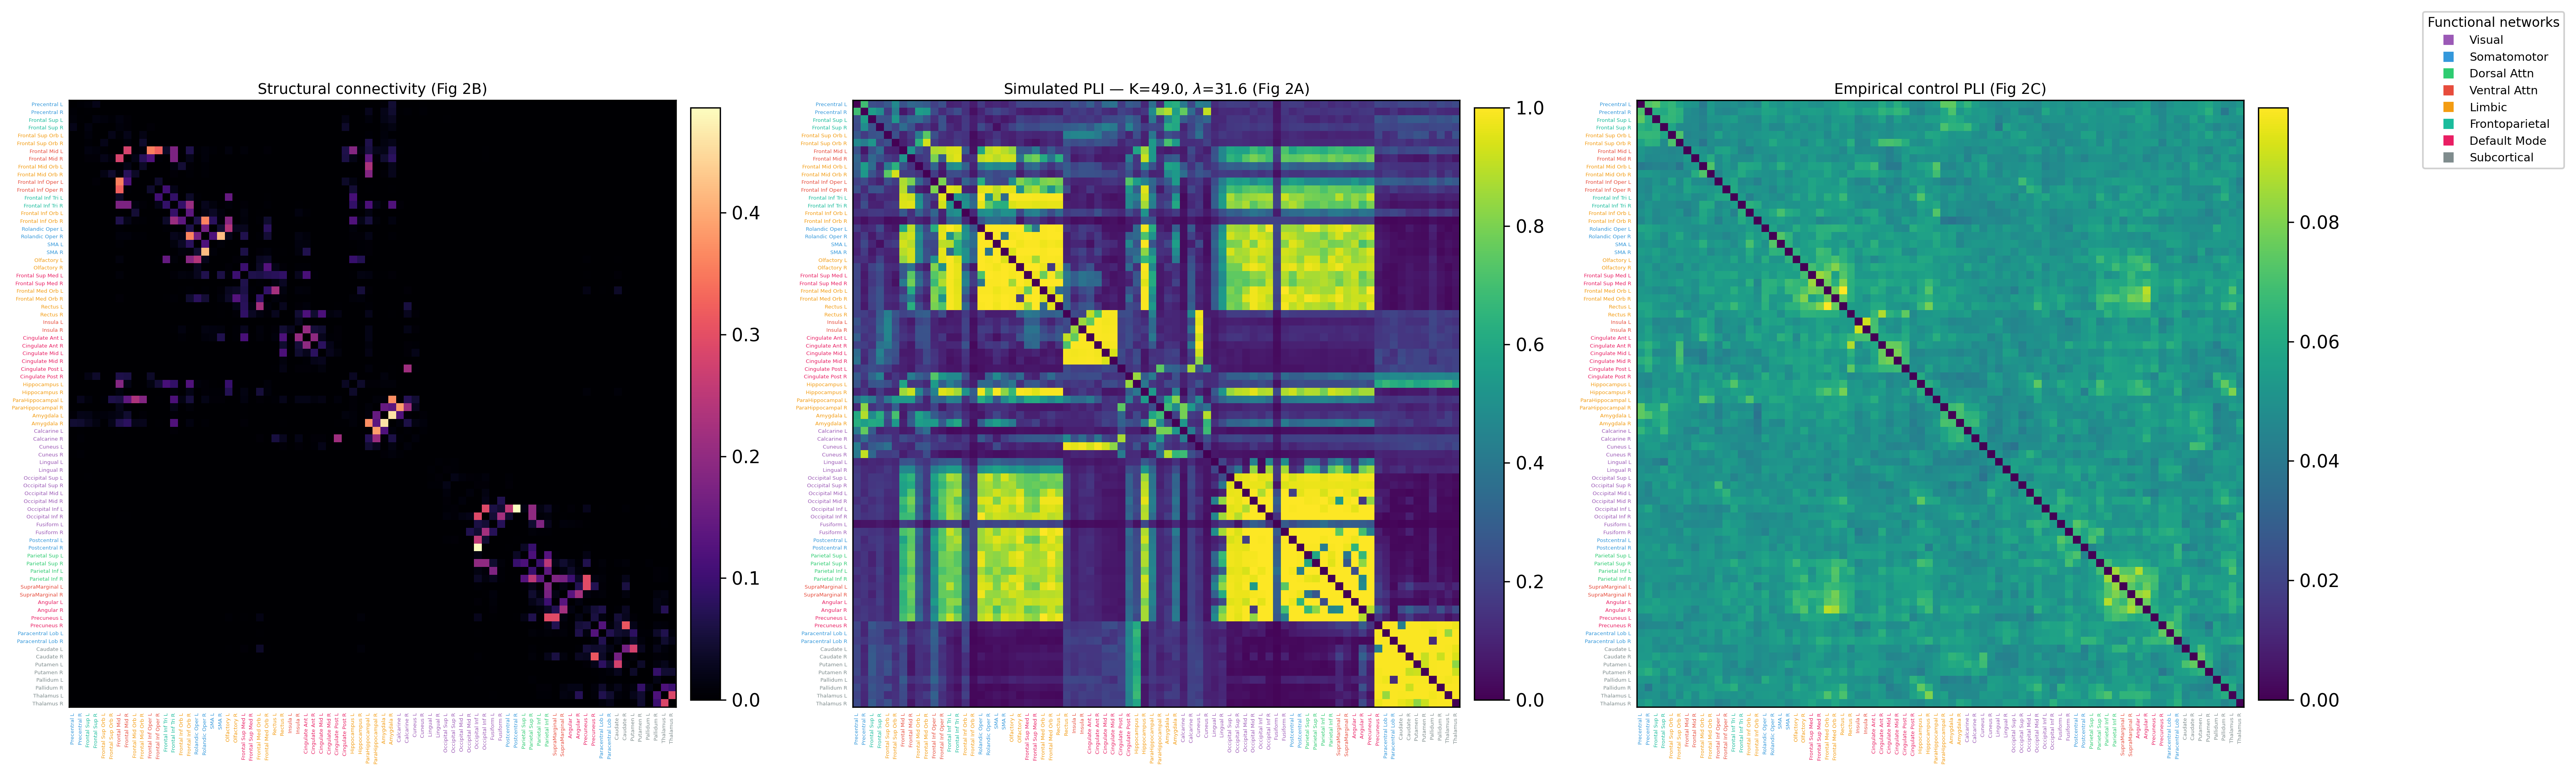
\includegraphics[width=0.95\textwidth]{../figures/hopf model/network stability/fig2_labelled_matrices.png}
    \caption{
    Empirical-scale network fitting. Shown are the empirical structural connectivity matrix, a best-fit simulated PLI matrix, and the empirical control PLI matrix. The simulated matrix reproduces broad block-structured organisation present in the empirical data, supporting the use of the coupled Hopf network as a coarse-grained model of large-scale functional connectivity.
    }
    \label{fig:network_matrices}
\end{figure*}

\begin{figure*}[t]
    \centering
    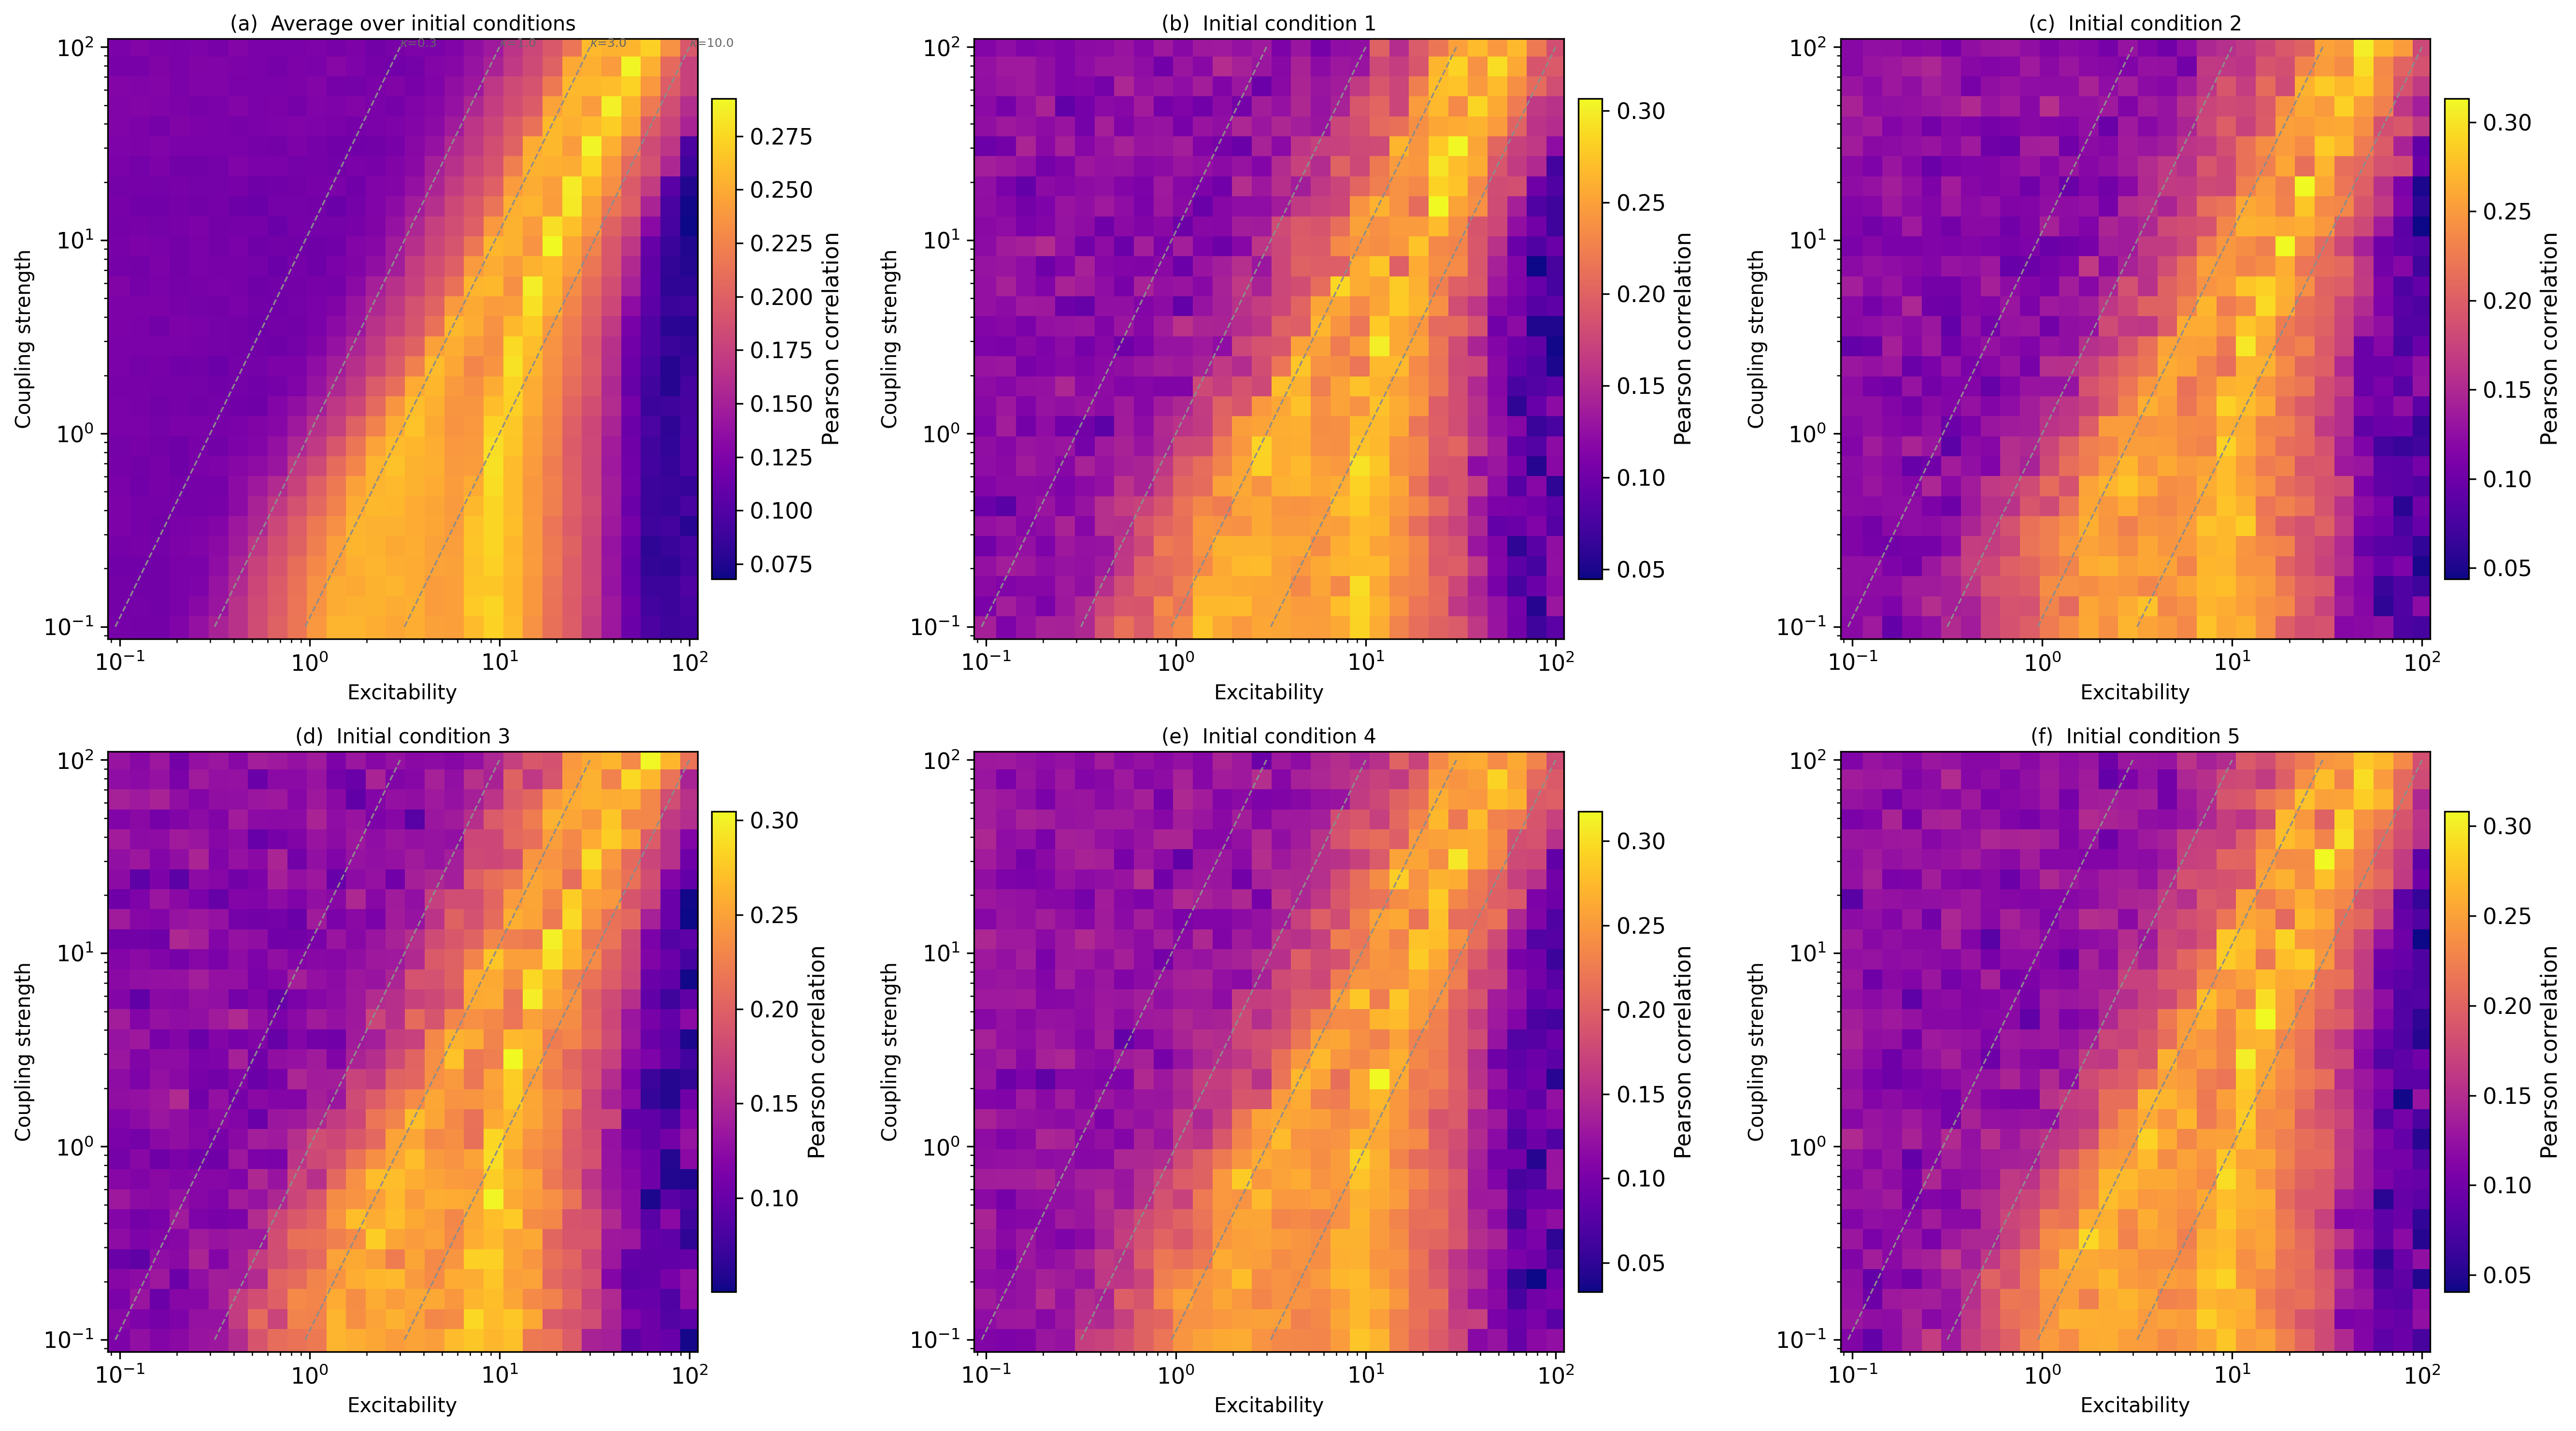
\includegraphics[width=0.95\textwidth]{../figures/hopf model/network stability/fig3_loglog_grid.png}
    \caption{
    Log--log parameter search for the empirical network model. Across multiple initial conditions, the best-fit region follows approximately diagonal bands corresponding to constant $\kappa = K/\sqrt{\lambda}$, indicating that the goodness of fit is largely controlled by the normalised coupling rather than by $K$ and $\lambda$ independently.
    }
    \label{fig:network_scaling}
\end{figure*}

\begin{figure*}[t]
    \centering
    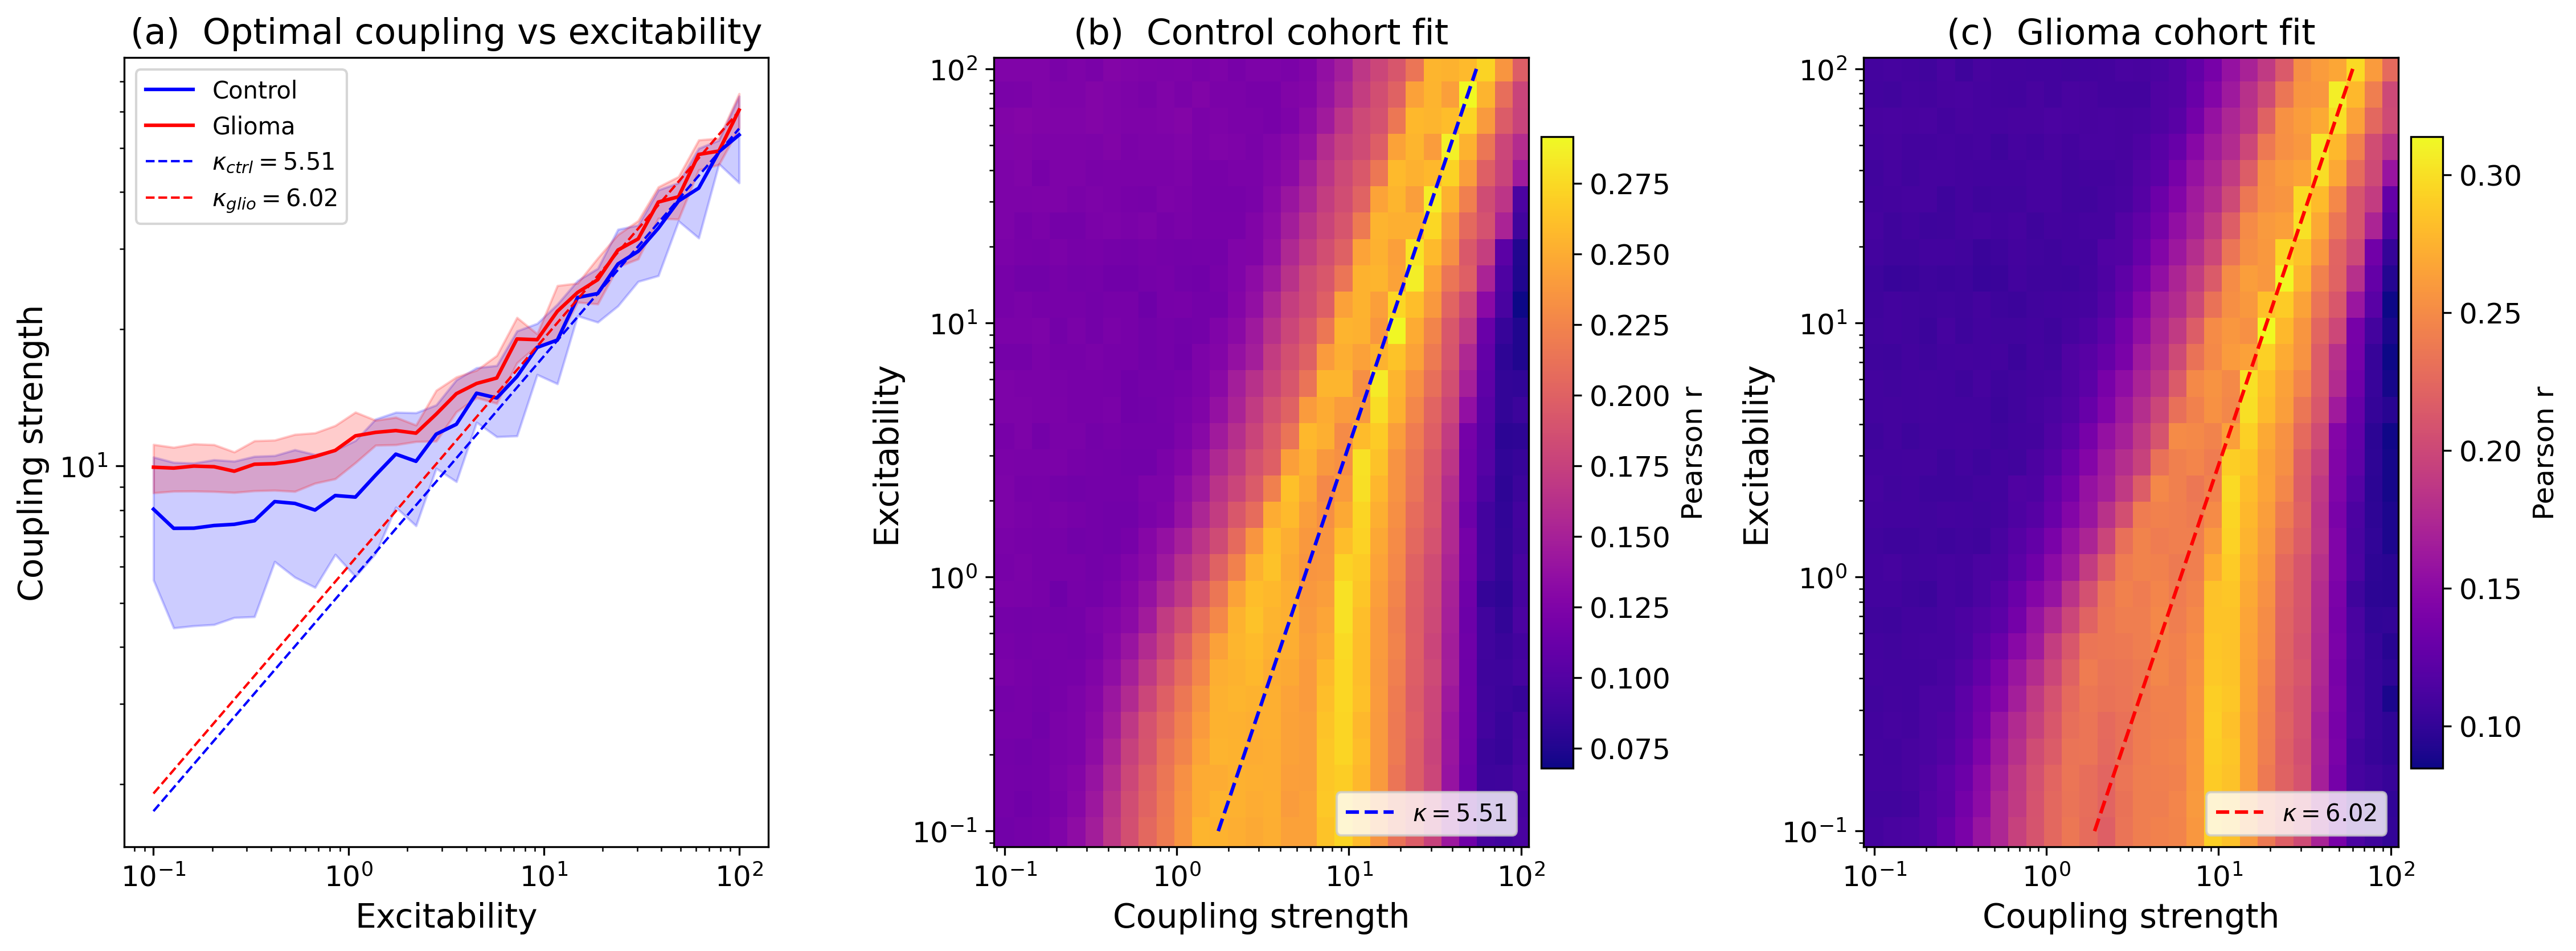
\includegraphics[width=0.95\textwidth]{../figures/hopf model/network stability/fig4_glioma_comparison.png}
    \caption{
    Comparison of fitted parameter landscapes for the control and glioma cohorts. The optimal coupling curve lies systematically above the control curve, corresponding to a larger fitted normalised coupling for the glioma cohort. This indicates a shift toward stronger global interactions in the glioma network dynamics.
    }
    \label{fig:network_glioma}
\end{figure*}

\begin{figure*}[t]
    \centering
    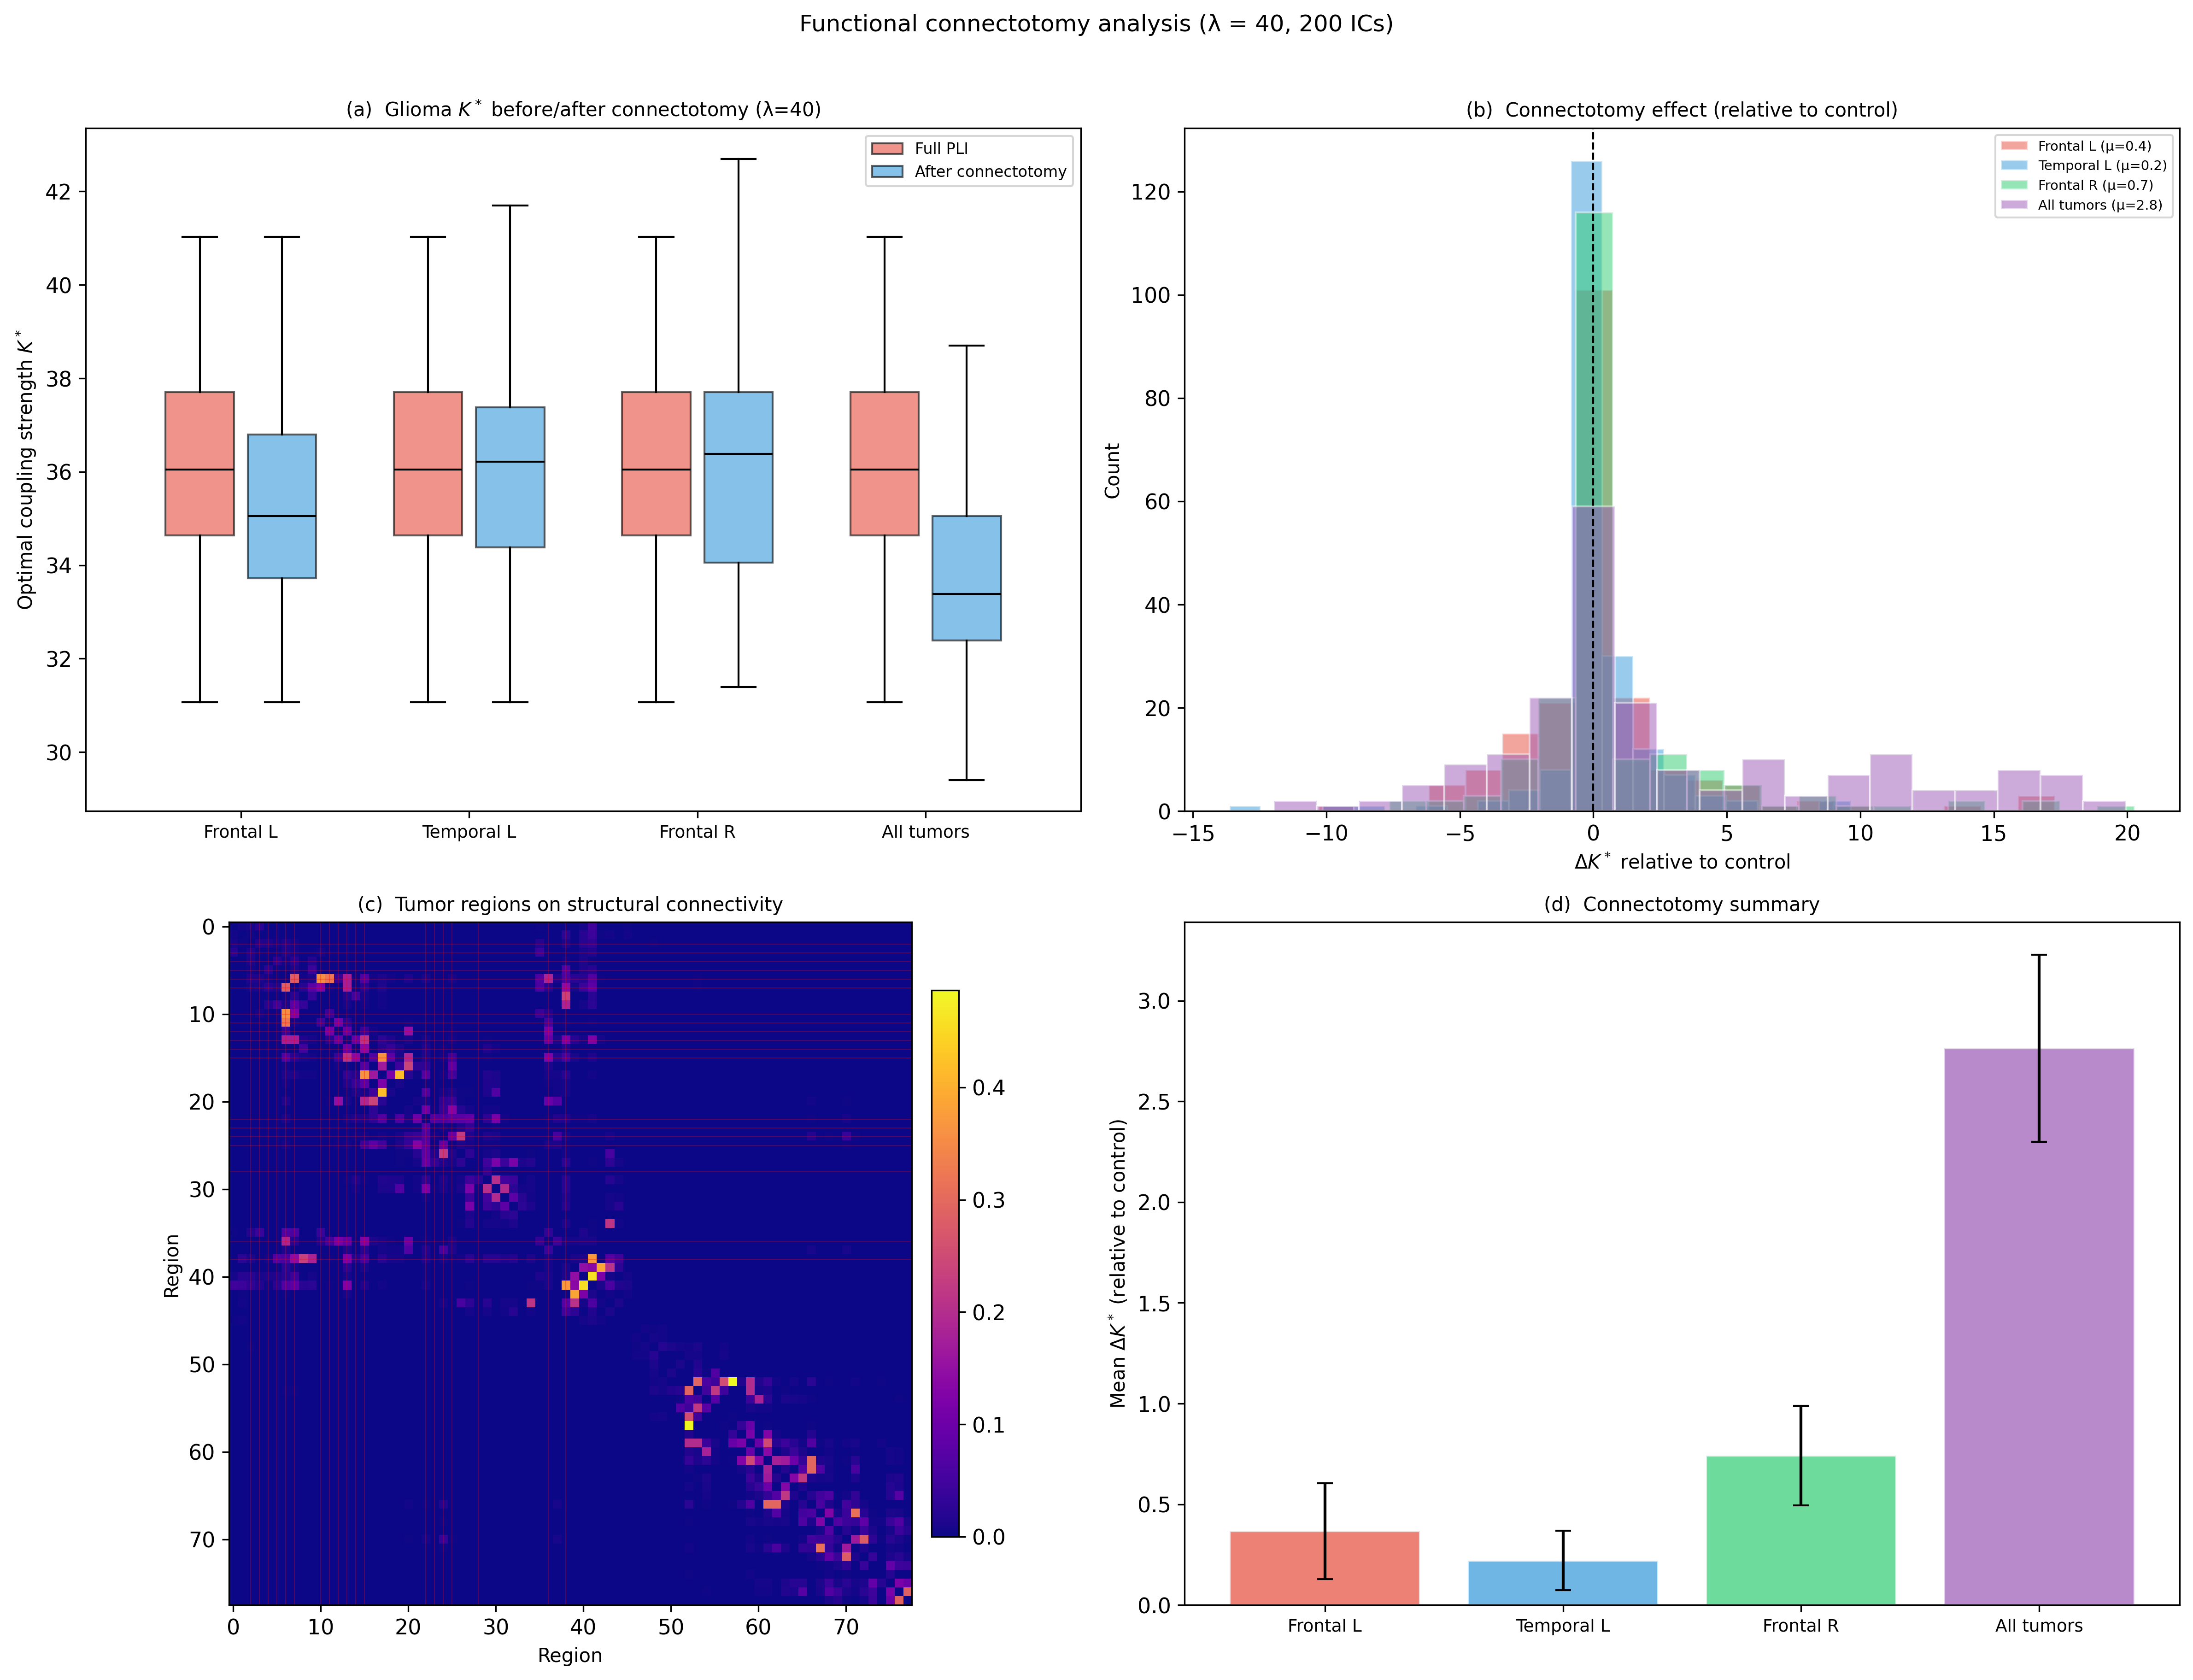
\includegraphics[width=0.95\textwidth]{../figures/hopf model/network stability/fig6_8_connectotomy.png}
    \caption{
    Functional connectotomy analysis. Removing tumour-related regions from the PLI comparison and refitting the model generally reduces the optimal coupling strength relative to the corresponding control comparison, indicating that tumour regions contribute to the elevated coupling observed in glioma fits.
    }
    \label{fig:network_connectotomy}
\end{figure*}




\subsection{Virtual lesioning atlas}
To extend the connectotomy analysis beyond the predefined tumour-region sets used in the original paper, we evaluated the lesioning effect of all 78 AAL regions on the fitted optimal coupling. The resulting region-wise atlas showed that lesioning effects were spatially heterogeneous rather than uniform across the brain (Fig.~\ref{fig:ranked_dk}). In the glioma fit, a subset of regions produced noticeably larger changes in the optimal coupling than the rest, whereas the control profile was comparatively flatter when shown in the same regional order. This indicates that the elevated coupling required to reproduce the glioma functional connectivity is driven disproportionately by specific regions rather than being distributed evenly across the network.
To isolate disease-specific effects, we compared the lesioning responses in glioma and control using the differential score
\[
\Delta K_i^{\mathrm{diff}}=\Delta K_i^{\mathrm{glioma}}-\Delta K_i^{\mathrm{control}}.
\]
The resulting differential atlas identified a subset of regions whose masking reduced the fitted coupling more strongly in glioma than in control (Fig.~\ref{fig:differential_atlas}). The strongest positive differential effects were concentrated mainly in frontal and medial regions, including bilateral medial orbital and superior medial frontal areas, together with posterior cingulate and a smaller number of occipital and parietal regions. In contrast, several sensorimotor, insular, and subcortical regions showed negative differential effects, indicating weaker or more control-like lesioning responses. Taken together, these results extend the original connectotomy analysis from grouped tumour regions to a region-resolved whole-brain map of candidate coupling drivers.

\subsection{Relation to structural connectivity}
We next asked whether the strongest virtual-lesioning effects could be explained by the structural importance of the affected regions. Degree and weighted strength were not significantly associated with lesioning effect size in either cohort (control: degree $\rho=0.07$, $p=5.28\times10^{-1}$; strength $\rho=-0.04$, $p=7.36\times10^{-1}$; glioma: degree $\rho=0.01$, $p=9.55\times10^{-1}$; strength $\rho=-0.05$, $p=6.81\times10^{-1}$; Fig.~\ref{fig:hubness_vs_dk}). By contrast, eigenvector centrality showed a significant positive association with lesioning effect size in both cohorts, with a stronger relationship in glioma than in control (control: $\rho=0.32$, $p=4.51\times10^{-3}$; glioma: $\rho=0.41$, $p=1.94\times10^{-4}$; Fig.~\ref{fig:hubness_vs_dk}). Thus, the strongest coupling drivers are not simply the nodes with the largest number or weight of connections, but are more closely related to globally influential regions in the structural network.
Overall, the extension suggests that the connectotomy effect reported in the original paper is not only recoverable at the level of grouped tumour regions, but can be resolved into a whole-brain atlas of region-specific coupling drivers, with the clearest glioma-specific effects emerging in a subset of structurally influential frontal and medial regions.
This regional pattern was also broadly consistent with the tumour-region grouping used in the original paper, supporting the interpretation that the strongest lesioning drivers overlap with tumour-associated regions.

\begin{figure*}[t]
    \centering
    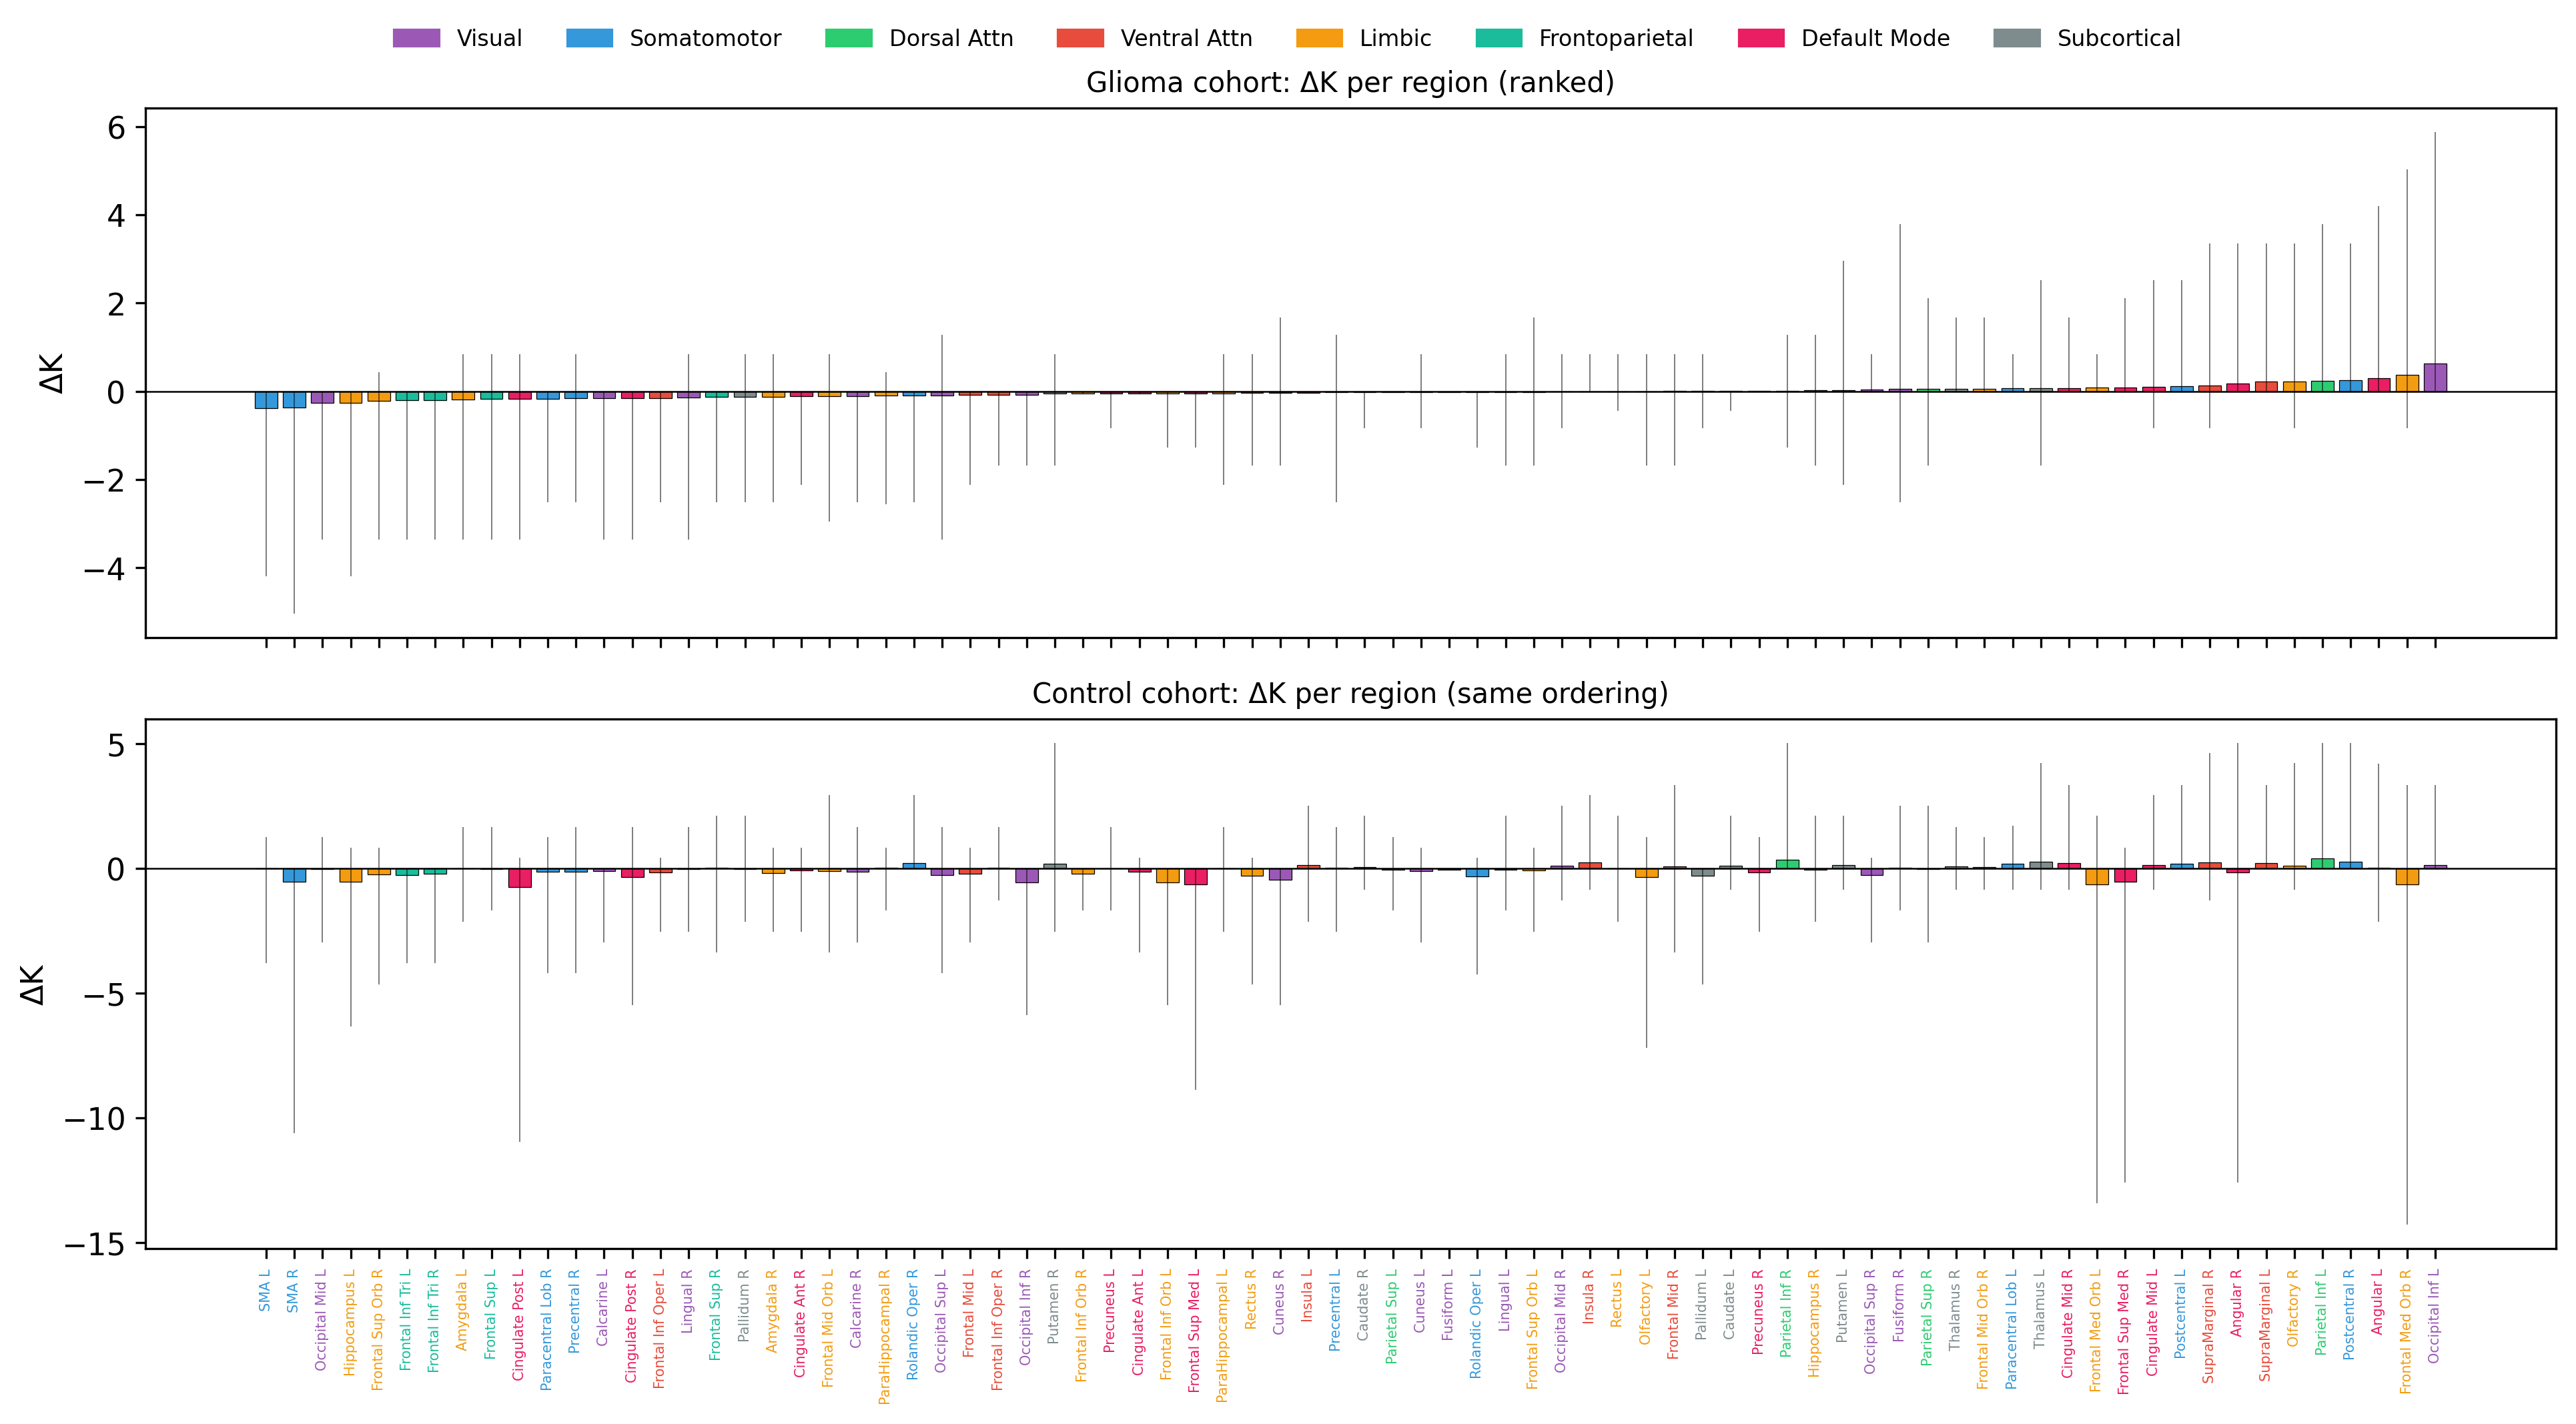
\includegraphics[width=\textwidth]{../figures/hopf model/virtual lesioning/fig1_ranked_dK.png}
    \caption{
    Region-wise virtual-lesioning effects on fitted coupling. Top: glioma cohort lesioning effect $\Delta K$ for all 78 AAL regions, ranked by effect size. Bottom: control-cohort lesioning effects shown in the same regional order. Regions are coloured by large-scale network affiliation. The glioma profile shows a more structured and regionally selective pattern than the control profile.
    }
    \label{fig:ranked_dk}
\end{figure*}

\begin{figure*}[t]
    \centering
    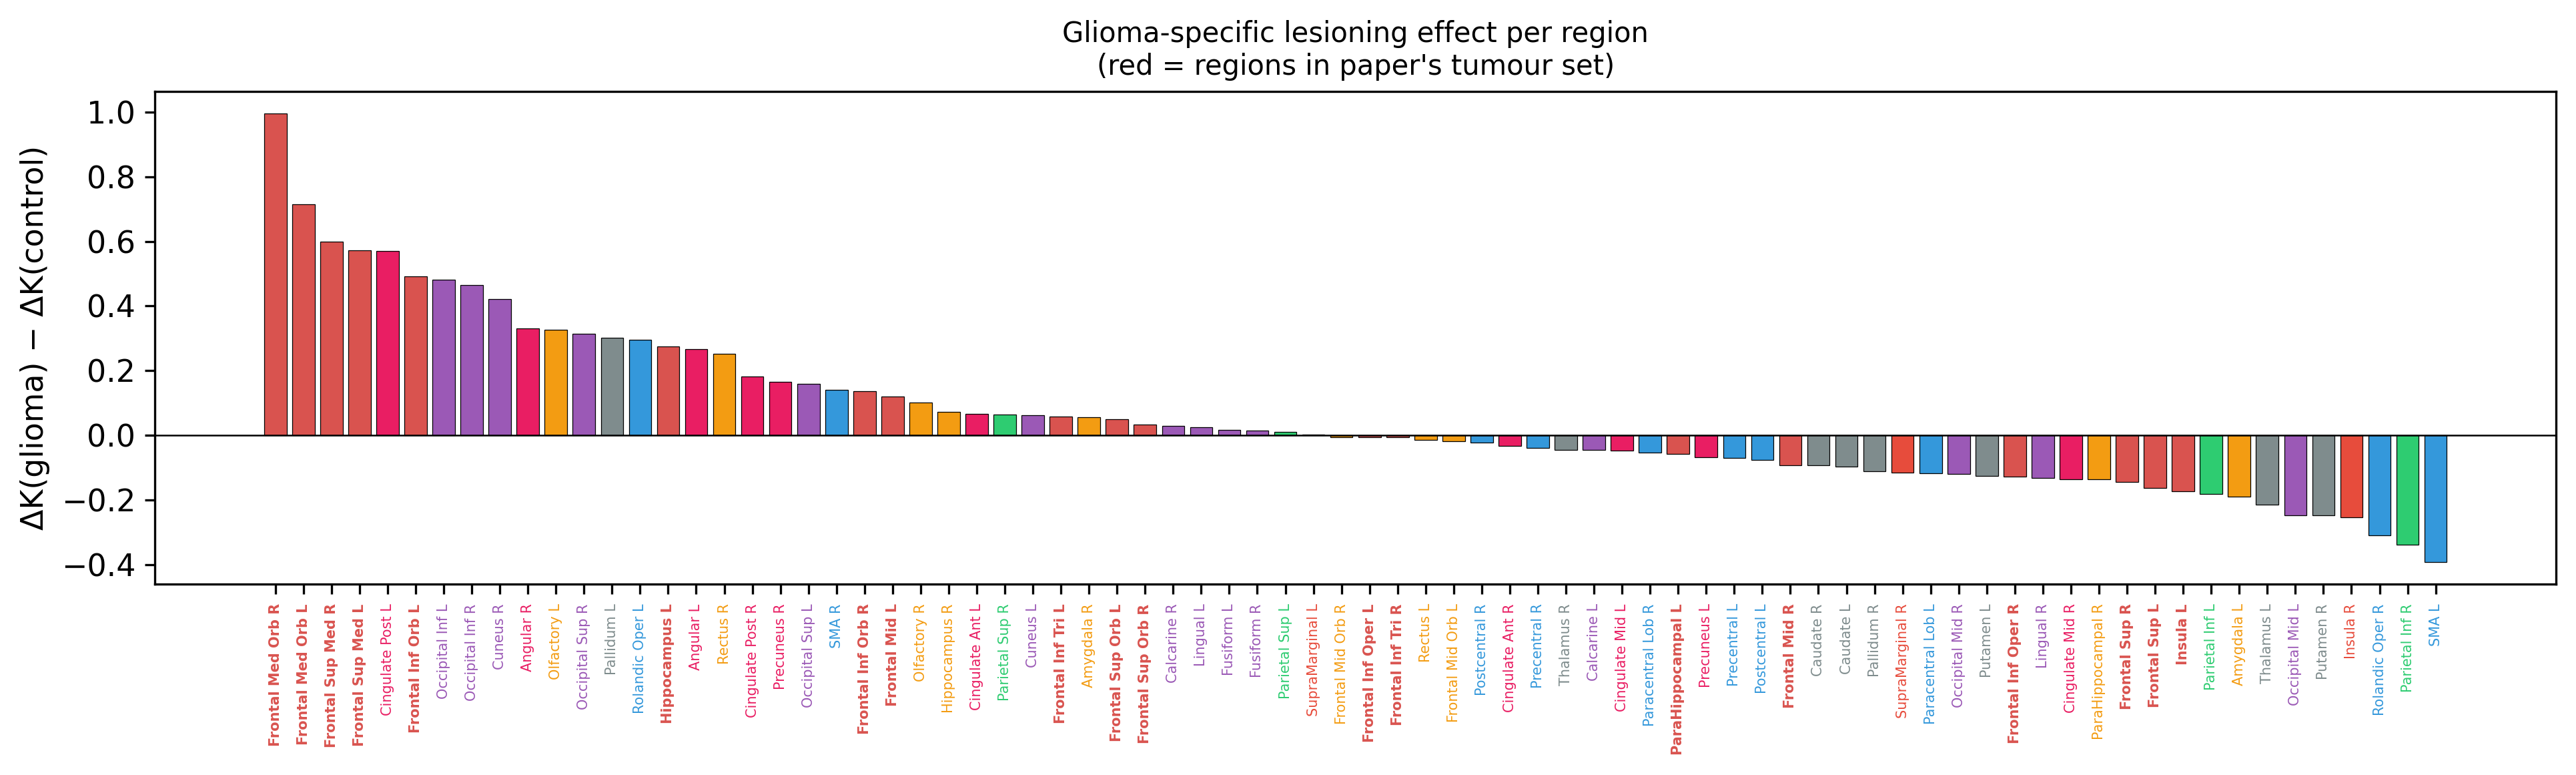
\includegraphics[width=\textwidth]{../figures/hopf model/virtual lesioning/fig3_differential_atlas.png}
    \caption{
    Glioma-specific virtual-lesioning effect per region, quantified by $\Delta K_i^{\mathrm{glioma}}-\Delta K_i^{\mathrm{control}}$. Red labels indicate regions belonging to the tumour-region set used in the original paper. Positive values indicate regions whose masking reduces fitted coupling more strongly in glioma than in control.
    }
    \label{fig:differential_atlas}
\end{figure*}

\begin{figure*}[t]
    \centering
    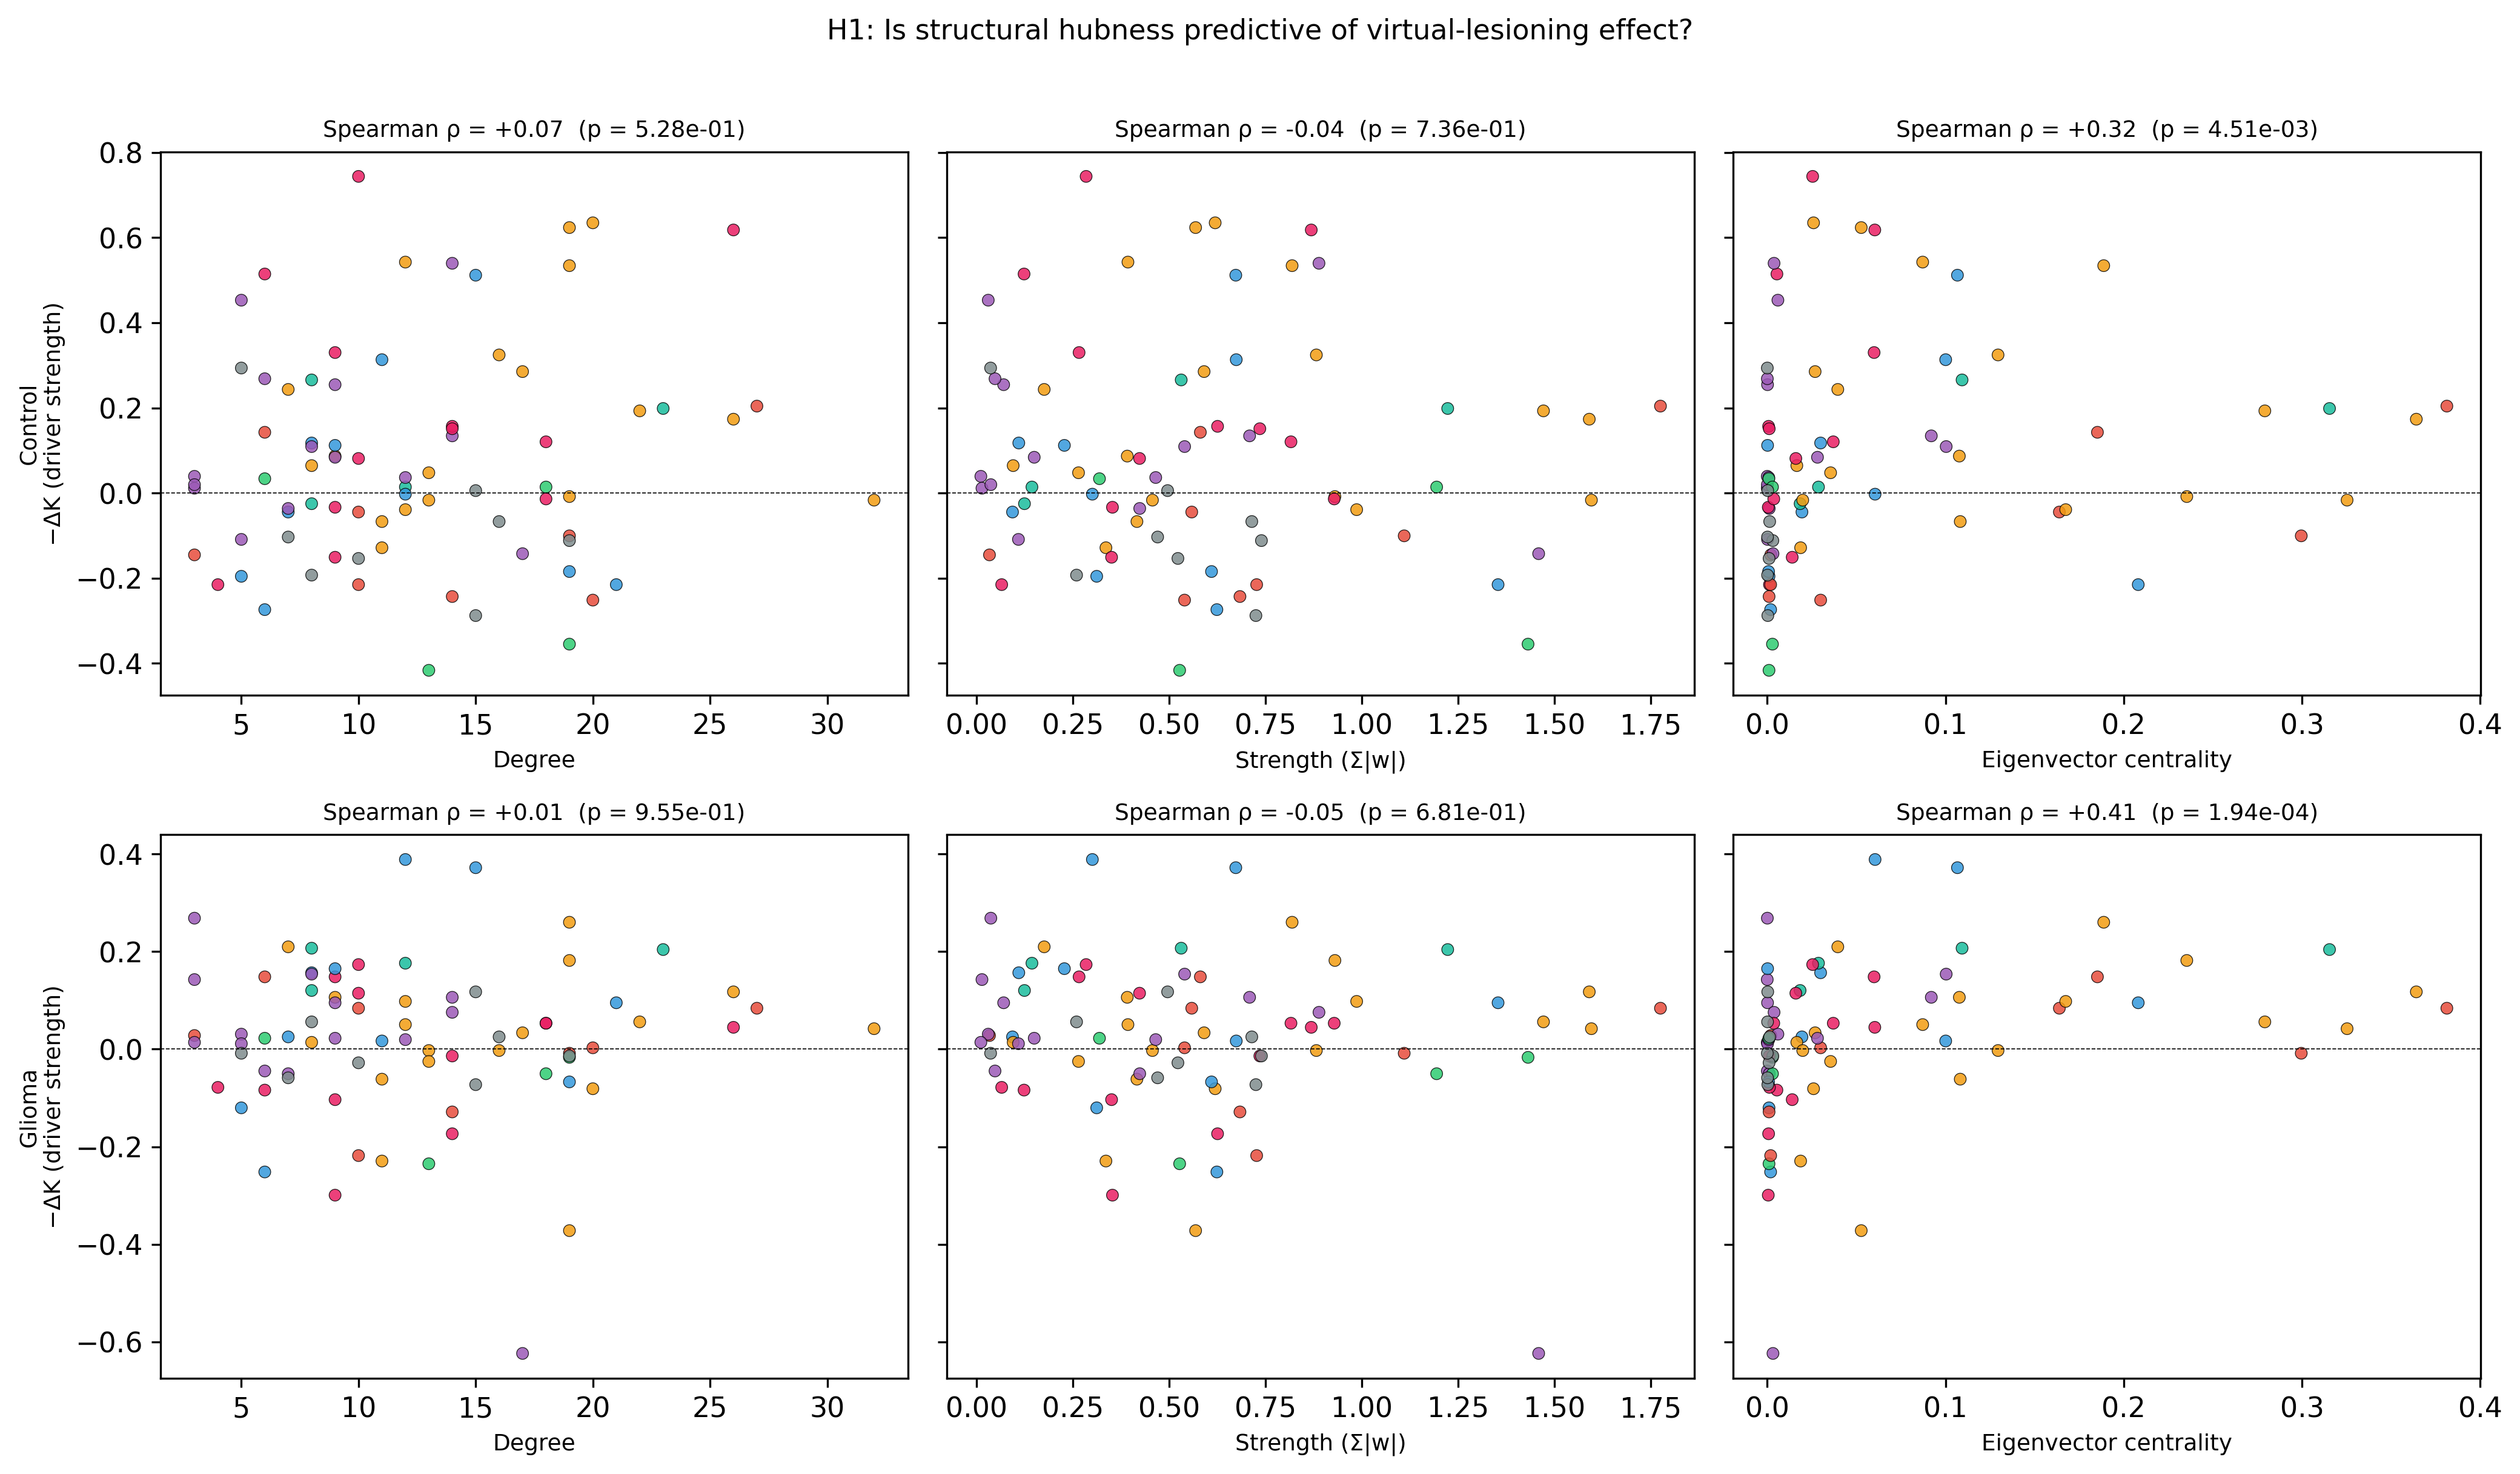
\includegraphics[width=\textwidth]{../figures/hopf model/virtual lesioning/fig4_hubness_vs_dK.png}
    \caption{
    Relationship between structural hubness and virtual-lesioning effect size. Degree and weighted strength show no significant association with lesioning effects, whereas eigenvector centrality is positively associated with lesioning effect size in both control and glioma fits, with a stronger relationship in glioma.
    }
    \label{fig:hubness_vs_dk}
\end{figure*}






\subsection{Structural connectivity perturbation}
We next tested whether directly damaging the structural connections of the strongest control coupling drivers would alter the fitted coupling in the control model. Using the virtual-lesioning atlas, the three most influential control regions were identified as left posterior cingulate cortex, left medial orbitofrontal cortex, and right medial orbitofrontal cortex. These regions were then subjected to graded structural perturbation in the empirical control connectome, as identified by their low mean $\Delta K$ values in the virtual-lesioning analysis.

Across all damage levels, the fitted optimal coupling remained fixed at
\[
K^{*}=0.38,
\]
and the fitted excitability remained fixed at
\[
\lambda^{*}=0.
\]
Thus, within the parameter grid explored in this perturbation analysis, progressive structural damage to these driver regions did not produce a measurable shift in the best-fitting model regime. The retained correlation landscapes likewise did not show an obvious systematic shift in the location of the high-fit region across damage levels. In particular, the perturbation did not drive the control fit toward a distinctly larger coupling value that would resemble the glioma-shifted regime observed in the main reproduction. However, given the relatively coarse parameter grid, smaller shifts in the optimal region may not be fully resolved. 

The goodness of fit changed only weakly across the dose-response sweep and exhibited no clear monotonic trend. The maximum Pearson correlation between simulated and empirical control PLI was $0.0098$ in the undamaged case, rose slightly to $0.0099$ at 25\% damage, dipped to $0.0087$ at 50\% damage, and then increased to $0.0101$ at 75\% damage and $0.0135$ at the strongest perturbation level. Although this suggests a small improvement in fit at the strongest perturbation levels, the effect size remained modest and did not coincide with any change in the fitted $(K,\lambda)$ optimum. Moreover, the absolute correlation values remained low across all conditions, indicating that the model fit in this perturbation setting was weak overall.

Taken together, these results indicate that, in the present perturbation implementation and parameter range, damaging the structural connections of the top control drivers was not sufficient to reproduce the elevated-coupling signature associated with glioma. The extension therefore provides only limited support for a simple anatomy-only explanation of the glioma-control difference, and suggests that either stronger perturbations, a wider parameter search, or more targeted region selection may be required to reveal a clearer structural dose-response effect.

\section{Discussion}
In this project, we reproduced the central dynamical findings of Alexandersen et al.~\cite{Alexandersen2025} and extended their connectotomy framework to a region-resolved virtual-lesioning atlas. At the reproduction level, our results support the main claim of the original paper: phase-based functional connectivity in the Hopf whole-brain model is governed primarily by the balance between interregional coupling and local excitability, rather than by either parameter independently. In particular, we recovered the approximate scaling relation $K \propto \sqrt{\lambda}$ and found that the best-fitting parameter region lies at positive values of $\lambda$, consistent with the original study. We further reproduced the shift toward higher fitted coupling in the glioma cohort and the connectotomy result that removing tumour-related regions from the fitting comparison tends to reduce the optimal coupling, supporting the interpretation that tumour-associated regions contribute to the elevated interregional influence observed in glioma.
A key implication of the reproduction is that parameter interpretation in whole-brain Hopf models must be treated carefully. The results do not suggest that the raw coupling parameter $K$ alone is the most meaningful descriptor of system behaviour. Rather, both the reduced-model analyses and the empirical network fitting indicate that the relevant quantity is the normalised coupling $\kappa = K/\sqrt{\lambda}$, which expresses the balance between global interactions and local oscillatory dynamics. This is important because it reframes the glioma-control difference not simply as ``more coupling,'' but as a shift in the relative contribution of interregional interactions compared with local excitability. In that sense, the pathology appears to alter the effective balance of scales in the model, increasing the extent to which global network interactions shape the observed functional connectivity.
The functional connectotomy analysis provides further support for this interpretation. In both the original paper and our reproduction, tumour-related regions were not removed from the network model itself, but from the comparison between simulated and empirical functional connectivity. The resulting decrease in fitted coupling after connectotomy suggests that these regions contribute disproportionately to the elevated coupling required to match the glioma data. At the same time, the effect is not uniform across patients or region groups, which is consistent with the heterogeneity of glioma and with the relatively small cohort size used in the original study. Therefore, the connectotomy result is best interpreted as evidence for a broad trend rather than a strictly localised or deterministic mechanism.
Our extension developed this idea further by replacing the predefined tumour-region sets with a systematic virtual-lesioning analysis over all 78 AAL regions. This showed that the connectotomy effect can be resolved into a region-wise atlas of coupling drivers. The lesioning effects were spatially heterogeneous: most regions had little influence on the fitted optimal coupling, while a smaller subset produced substantially larger shifts. Moreover, the glioma fit showed a more structured and selective lesioning profile than the control fit, and the differential atlas identified a subset of regions whose contribution to coupling was stronger in glioma than in control. These findings suggest that the elevated coupling observed in glioma is not a diffuse whole-brain effect, but is instead driven disproportionately by specific regions.
An important result of the extension is that the strongest lesioning effects were associated with eigenvector centrality, but not with degree or weighted strength. This indicates that the regions acting as coupling drivers are not simply those with the largest number of connections or the greatest total connection weight. Instead, they are more closely related to globally influential nodes in the structural network. This distinction matters because it suggests that the connectotomy effect is not reducible to a trivial hubness effect. The disease-specific coupling drivers appear to be embedded in important parts of the network architecture, but their contribution is still selective rather than generic. In other words, glioma-related alterations may preferentially amplify the role of structurally influential regions in shaping whole-brain phase synchronisation.
Taken together, these results extend the conclusions of Alexandersen et al.~\cite{Alexandersen2025} in two ways. First, they support the original interpretation that tumour-associated pathology shifts whole-brain dynamics toward stronger effective interregional coupling. Second, they show that this shift can be spatially refined into a region-wise atlas of candidate coupling drivers, with the clearest glioma-specific effects emerging in a limited subset of frontal and medial regions. This suggests that glioma-related alterations in functional connectivity are not only global in character, but are also shaped disproportionately by specific structurally influential regions.


\section{Limitations}
Several limitations should be considered when interpreting these results. First, the Hopf whole-brain model is a simplified phenomenological description of neuronal dynamics, so fitted parameters should be interpreted as model-level descriptors rather than direct physiological quantities. Second, both the reproduction and the extension are based on static, phase-based functional connectivity derived from PLI, and therefore do not capture temporal fluctuations or more complex metastable dynamics. Third, the framework inherits simplifying assumptions from the original study, including the use of a fixed structural connectome, thresholded PLI matrices, and predominantly global parameters, which may reduce sensitivity to subject-specific or region-specific mechanisms. Finally, the virtual-lesioning atlas is a model-based measure of how strongly masking a region changes fitted coupling, and should not be interpreted as a direct causal map of tumour influence in vivo.

\section{Future directions}


\section{Conclusion}
In this project, we reproduced the main findings of Alexandersen et al.~\cite{Alexandersen2025} using a Hopf whole-brain model of phase-based functional connectivity. In particular, we recovered the approximate scaling relation between coupling strength and excitability, showing that the model dynamics are organised primarily by the normalised coupling $\kappa = K/\sqrt{\lambda}$, and we reproduced the shift toward higher fitted coupling in the glioma cohort. We also recovered the connectotomy result that removing tumour-related regions from the fitting comparison tends to reduce the optimal coupling, supporting the interpretation that tumour-associated regions contribute to the elevated interregional influence observed in glioma.
Building on this reproduced framework, we extended the analysis with a region-wise virtual-lesioning atlas. This showed that the coupling abnormalities identified by the original connectotomy analysis are not distributed uniformly across the brain, but are driven disproportionately by a subset of regions. Moreover, the strongest lesioning effects in glioma were associated more closely with eigenvector centrality than with degree or weighted strength, suggesting that the most important coupling drivers are globally influential regions rather than simply the most locally connected nodes.
Overall, these findings support the view that glioma-related alterations in whole-brain dynamics reflect a shift in the balance between local oscillatory activity and large-scale network interactions. More broadly, they show that connectotomy-style perturbation analyses can be extended beyond predefined tumour regions to generate region-resolved maps of candidate coupling drivers, providing a useful framework for future studies of how local pathology reshapes global brain dynamics.

\begin{thebibliography}{99}
\bibitem{Deco2011}
G. Deco, V. K. Jirsa, and A. R. McIntosh, “Emerging concepts for the dynamical organization of resting-state activity in the brain,” Nature Reviews Neuroscience, vol. 12, no. 1, pp. 43–56, 2011.
\url{https://doi.org/10.1038/nrn2961}
\bibitem{Deco2014}
G. Deco, and M. L. Kringelbach, “Great expectations: using whole-brain computational connectomics for understanding neuropsychiatric disorders,” Neuron, vol. 84, no. 5, pp. 892–905, 2014.
\url{https://doi.org/10.1016/j.neuron.2014.08.034}
\bibitem{Cabral2011}
J. Cabral, E. Hugues, O. Sporns, and G. Deco, “Role of local network oscillations in resting-state functional connectivity,” NeuroImage, vol. 57, no. 1, pp. 130–139, 2011.
\url{https://doi.org/10.1016/j.neuroimage.2011.04.010}
\bibitem{Freyer2011}
F. Freyer, J. A. Roberts, R. Becker, P. A. Robinson, P. Ritter, and M. Breakspear, “Biophysical mechanisms of multistability in resting-state cortical rhythms,” The Journal of Neuroscience, vol. 31, no. 17, pp. 6353–6361, 2011.
\url{https://doi.org/10.1523/JNEUROSCI.6693-10.2011}
\bibitem{Alexandersen2025}
C. G. Alexandersen, L. Douw, M. L. M. Zimmermann, C. Bick, and A. Goriely, "Functional connectotomy of a whole-brain model reveals tumor-induced alterations to neuronal dynamics in glioma patients," Network Neuroscience, vol. 9, no. 1, pp. 280--302, 2025.
\url{https://doi.org/10.1162/netn_a_00426}

\end{thebibliography}



\end{document}
